\documentclass[conference]{IEEEtran}
\IEEEoverridecommandlockouts
% The preceding line is only needed to identify funding in the first footnote. If that is unneeded, please comment it out.
\usepackage{cite}
\usepackage{amsmath,amssymb,amsfonts}
\usepackage{graphicx}
\usepackage{textcomp}
\usepackage{xcolor}
\usepackage[back-end=biber, style=ieee]{biblatex}
\usepackage{algorithm} 
\usepackage{algpseudocode} 
\addbibresource{refs.bib}
\begin{document}

\title{IoT Traffic Management System for Autonomous Vehicles}

\author{\IEEEauthorblockN{Rohit Singh}
\IEEEauthorblockA{\textit{Electrical Engineering} \\
\textit{University of Waterloo}\\
Waterloo, Ontario \\
rkochhar@uwaterloo.ca}
\and
\IEEEauthorblockN{Vojdan Bojcev}
\IEEEauthorblockA{\textit{Electrical Engineering} \\
\textit{University of Waterloo}\\
Waterloo, Ontario \\
vbojcev@uwaterloo.ca}
}

\maketitle
\thispagestyle{plain}
\pagestyle{plain}

\begin{abstract}
This document is a model and instructions for \LaTeX.
This and the IEEEtran.cls file define the components of your paper [title, text, heads, etc.]. *CRITICAL: Do Not Use Symbols, Special Characters, Footnotes, 
or Math in Paper Title or Abstract. \cite{Chong}\cite{Rizwan}\cite{Avetifipour}\cite{GOTTLICH}\cite{Ghena}.
\end{abstract}

\section{Introduction}

With the population of city centres rapidly increasing, the number of vehicles on the road is quickly becoming unsustainable for the current infrastructure. Densely populated cities such as Los Angeles and New York have become notorious for their gridlock and traffic, and there is little evidence to suggest that this problem will relent any time soon. 

While autonomous vehicles (AVs) propose a solution to the causes of traffic due to human-error, the larger issue comes from the non-dynamic implementation of traffic control systems such as stop lights. Theses systems can be seen as stateful controls that switch state to route traffic in a certain way. Despite the fact that the state of a given traffic light directly affects the traffic at another, these systems are largely isolated and do not typically communicate with each other. Because of this, traffic in one direction can become highly backed up while opposing traffic moves freely. 

In this work, we aim to propose a novel solution that transforms traditional traffic networks into dynamic sensor networks that communicate traffic flow information to autonomous vehicles within the network. Our proposed solution would allow traffic lights to act as communicating beacons, relaying information about real-time traffic flow to the path planning systems of autonomous vehicles to allow them to adopt the ideal route to reach their target destination.

\section{Literature Review}
\section{Experiment Methodology}



\subsection{Modelling of Transport Networks}\label{sec:modelling}

For our experiment, we need to create a model that can represent traffic flow between intersections. To accomplish this, we use a directed graph with intersections represented by nodes and traffic flow parameters representing the weights of connecting edges. Edges between nodes are uni-directional, which allows for one-way traffic flow to be modelled by a single edge or two-way traffic flow to be modelled by two edges. Each edge has an associated \textit{source} node (node from which traffic flows) and an associated \textit{sink} node (node to which traffic flows). The nodes serve as beacon points to communicate traffic data collected by the edges across the network to the AVs passing through each intersection.

\subsection{Traffic Flow (Edge) Modelling}\label{sec:edge}

In the modelling of the edges of our graph, we must characterize edges with relevant parameters that impact traffic flow. Therefore, we load the edges with the following information:

\begin{itemize}
    \item \textbf{Length}, $L$: This parameter is a floating point integer which represents the length of the edge (distance between the source and sink nodes) in kilometres. This is a metric of importance as it provides information (along with speed limit) as to the ideal time for a vehicle to complete travel along this path.
    \item \textbf{Speed Limit}, $v$: This parameter is a integer which represents the ideal \textit{maximum speed} a vehicle maintains along this path in kilometres per hour. We are operating under the assumption that the speed limit is not violated by vehicles in the system, and that the speed limit is a constant across an entire edge.
    \item \textbf{Number of Vehicles}, $N$: This parameter is an integer which represents the number of vehicles travelling on the edge at a given moment in time. The higher this number, the more congestion occurs, resulting in reduced traffic flow.
    \item \textbf{Minimum Travel Time}, $t_{min}$: This parameter is an integer which represents the ideal time it takes for a vehicle to complete a trip across an edge, in seconds. This parameter is calculated by the simple equation: 
    \begin{equation}
        t_{min} = \frac{L}{v} \times 3600
    \end{equation}
    \item \textbf{Actual Travel Time}, $t_{real}$: This parameter is an integer which represents the actual time takes for a vehicle to complete a trip across an edge. This is a calculated parameter which is a function of the number of vehicles, length, and the minimum travel time of the edge. In modelling the function that governs this parameter, we make the following assumptions:
    \begin{itemize}
        \item The average length of vehicles along the edge is 5 meters \cite{carsize}
        \item When cars get within 10 meters of each other, their speed decreases due to braking events at the lead vehicle causing a \textit{concertina effect}, in which differences in vehicle control system response times causes cascading delays along chains of vehicles. To model this effect, we determine the average distance between vehicles (given in units of meters per vehicle) with the following equation:
        \begin{equation}
            d = \frac{L - 5N}{N} 
        \end{equation}
        From this definition of $d$, we can define the actual speed due to traffic delays caused by a large volume of traffic, $v_{real}$. $v_{real}$ is inversely proportional to the square $d$, since the smaller the distance between cars, the more compounding delays are experienced across the vehicles on the edge. We define $v_{real}$ as follows:
        \begin{equation}\label{eq:v-real}
            v_{real} = 
        \left\{ \begin{array}{ll}
            v & d > 10 \\
            v(1 - \frac{1}{d}) & 10 \ge d > 1 \\ 
            1 & \text{otherwise}
        \end{array} \right.
        \end{equation}
        This equation is an accurate model for slow-down among vehicles due to large volumes of traffic, as we see a sharp decrease in $v_{real}$ as $d$ approaches values smaller than $2$ meters, which can be interpreted as the significant decrease in speed during bumper-to-bumper traffic. 
    \end{itemize}
    From equation \ref{eq:v-real}, we define $t_{real}$ as:
    \begin{equation}
        t_{real} = \frac{L}{v_{real}}\times 3600
    \end{equation}
    \item \textbf{Congestion}, $C$: This parameter is the key metric in controlling the states of the nodes, and is calculated by the equation:
    \begin{equation}
        C = \frac{t_{real}}{t_{min}} = \frac{v}{v_{real}} = \frac{v}{v(1 - \frac{1}{d})} = \frac{1}{1-\frac{N}{L-5N}}
    \end{equation}
    From this, we can see that when there is adequate space between vehicles on the road, $C = 1$, and as the number of vehicles on the edge increases (and consequently the space between vehicles on the road decreases), $C \to \infty$.
    
\end{itemize}

\subsubsection{Traffic Intersection (Node) Modelling}\label{sec:node}

As mentioned earlier in section \ref{sec:modelling}, our nodes are communicating beacons that relay traffic information to AVs within the network. The communication between the node and a given AV in the network closely follows the pseudo-code function shown in algorithm \ref{code:vtn-comm}. 

\begin{algorithm}
	\caption{Vehicle-to-Node Communication}\label{code:vtn-comm}
	\begin{algorithmic}[1]
	    \If {communication established}:
	        \State AV sends node target location
	        \State Node computes optimized path
	        \State Node sends AV optimized path to target
	        \State AV path planning system updates route
	    \EndIf
	\end{algorithmic} 
\end{algorithm}

Notice that in this system, our nodes are responsible for the computation of the ideal path, rather than the AV's computer. This is to prevent the transmission of large data packets to the AV, since the only data transmitted is the location of the next node the AV must travel to.

Since we must communicate the locations of the nodes to the autonomous vehicle, each node must store a record of its latitude and longitude. This allows the target location to be communicated in a way that can be interpreted by the majority of path-planning systems used for AVs \cite{pathplanning}.

The method by which the node determines the optimized route is by running Djikstra's algorithm \cite{clrs} to determine the shortest path in terms of the real time measurement between the current node and the target node communicated by the AV. This implementation of Djikstra's algorithm is outlined in algorithm \ref{code:djikstras}. 

\begin{algorithm}
	\caption{Path of Minimum Travel Time Using Djikstra's}\label{code:djikstras}
	\begin{algorithmic}[1]
	    \State TODO: Fill this out
	\end{algorithmic} 
\end{algorithm}

\subsection{Discrete Event Simulator Implementation}

Now that our graph definitions are complete, we must implement a way to model the behavior of the AVs when they are travelling along an edge. To do this, a \textit{discrete event simulator} (DES) is implemented. The DES serves as the clock of the entire simulation environment, maintaining a global reference time across all nodes, edges and vehicles. Since our edges are defined by speed, length, and travel time, we can mathematically define the average speed of any vehicle along a given edge at a given moment. From this calculation, we are able to determine the amount of time left before the vehicle completes a trip along the given edge and begins a trip across another. 

The simulator is given a topological graph $G$ from the definition of various nodes and their connecting edges. The speed limit and distance of each edge is declared at edge creation, from which the remaining parameters outlined in section \ref{sec:edge} are derived. Once the network is defined, AVs must be added to the edges to model congestion and traffic flow. This is done by either creating a number of vehicles, $N$ with declared or randomly assigned start and end nodes, and adding them to a collection of \textit{waiting} vehicles, $W$. Once the simulation starts, these vehicles are gradually added into the system by random selection, moving them from the \textit{waiting} collection to the \textit{travelling} collection $T$, and their \textit{baseline path} is computed using Djikstra's algorithm with the minimizing edge weight being \textit{minimum travel time}. This baseline path simulates routing uninformed by traffic flow, and serves as the ground truth for which the efficiency of our model is compared against. Once each AV is deployed into the graph, they travel along every edge in their path, with their trip progress tracked by the global reference time $t$ maintained by the simulator. Once the vehicles have traversed all the edges in their route, we determine that they have reached their target node and they are added to the \textit{completed} collection, $C$. Once all vehicles are added to the completed collection the ground truth results are collected. This process is outlined in the pseudo-code function shown in algorithm \ref{code:baselineSimulation}

\begin{algorithm}
	\caption{Baseline Simulation}\label{code:baselineSimulation}
	\begin{algorithmic}[1]
	    \State $G \gets \text{Nodes}, \text{Edges}$
	    \State $W \gets \text{addVehicles}(N)$
	    \State $T \gets \text{[ ]}$
	    \State $C \gets \text{[ ]}$
	    \While{$\text{len}(W) \ne 0 \text{ and } \text{len}(C) \ne \text{N}$}
	        \If{$\text{len}(W) \ne 0$}
	            \If{$t \mod 10 = 0$}
	                \State $v$ = random($W$)
	                \State getBaselinePathInfo($v$)
	                \State $W$.remove($v$)
	                \State $T \gets v$
	            \EndIf
	        \EndIf
	        \For{$v \in T$}
	            \If{$v$ is done on current edge}
	                \If{$v$ has traversed path}
	                    \State $C \gets v$
	                    \State $T$.remove($v$)
	                \Else
	                    \State setNextEdge($v$)
	                \EndIf
	            \EndIf
	        \EndFor
	       \State $t = t + 1$
	    \EndWhile
	\end{algorithmic} 
\end{algorithm}

\subsection{Experimental Network}

To validate the performance of our models in simulations that closely resemble the real world. To accurately simulate the behavior of our model in various situations, we have designed multiple graphs to simulate different types of traffic networks found in the real world.

\subsubsection{General Performance}

First, the graph designed in figure \ref{fig:testNetwork} was implemented to test our model's performance in a general network comprised of a variety of roads.

\begin{figure}
    \centering
    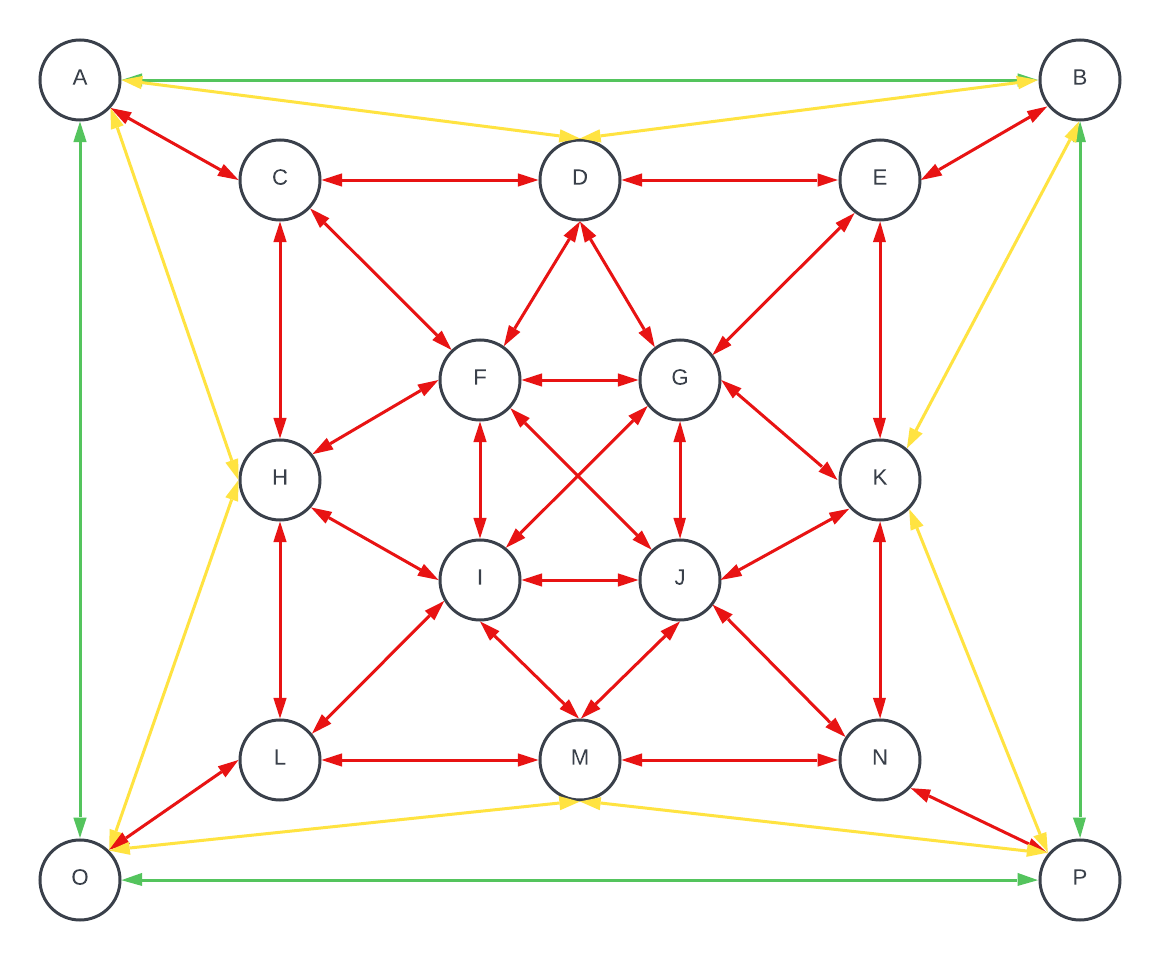
\includegraphics[scale=0.20]{captures/testNetwork.png}
    \caption{Caption}
    \label{fig:testNetwork}
\end{figure}

This network was designed to validate the general performance of our models across three main types of roads making up typical traffic networks:

\begin{enumerate}
    \item \textbf{Highway Roads}: These roads are represented by the green edges in our graph. They are characterized by their high speeds and long distances, with each edge of this type having $L = 40$km and $v = 110$ kph.
    \item \textbf{Rural Roads}: These roads are represented by the yellow edges in our graph. They are characterized by their medium-high speeds and long distances, with each edge of this type having $L = 20$km and $v = 80$kph.
    \item \textbf{City Roads}: These roads are represented by the red edges in our graph. They are characterized by their low speeds and short distances with many connecting nodes. Each edge of this type has $L = 10$km and $v = 30$kph.
\end{enumerate}

These three types of edges have varying degrees of susceptibility to congestion. Highway roads are designed to prevent congestion, as they have no intersections across their length, instead opting for on-ramps and off-ramps as traffic exchanges. This, in theory, creates a road in which traffic flow remains high and traffic is not an issue. However, this results in a large amount of traffic occupying these roads, resulting in heavy volumes of vehicles condensed together. This results in the \textit{concertina effect} discussed in section \ref{sec:edge}, causing braking delays to propagate through chains of vehicles close to one another resulting in a slow-down along the edge, as modelled by equation \ref{eq:v-real}. Rural roads often consist of longer stretches of medium speed roads with minimal intersections, and depending on the volume of traffic, can be viable alternatives to highway roads. Finally, city roads are highly prone to congestion, and typically contain a large amount of intersections controlled by traffic lights that result in significant slow-downs.

For the baseline, unoptimized result, we assume the cars are first routed by the minimum path determined by ideal travel time, which is the travel time assuming that there is no congestion and optimum travel flow. Initially, this will result in ideal traffic flow, but as a large volume of vehicles plan their paths this way, there will be a large build up of congestion along the paths with the ideal minimum time, causing congestion and slow-downs. 

\section{Experimental Results}

\printbibliography
\end{document}

\iffalse %NOTES/BRAINSTORMING

CHONG:

Discuss different network topologies: on-road, on-vehicle, or hybrid sensors. Discuss viability of having several wireless sensors at each intersection with one base station per intersection. Base stations can either be subservient to a master station or compute the optimization in a distributed manner. 

Goal of optimization is to minimize unused green-light time. Optimization is based on local load (single-intersection) but also must consider downstream (at least adjacent) intersections as well. Flat-hierarchy/local computation architectures could be better for local optimization where only 1-hop adjacent intersections are considered whereas multi-leveled/globally-computed architectures could be better for city-wide computations.

Generally, traffic algorithms are designed assuming a perfect network (i.e established city wifi/ethernet) which means state knowledge can be always known and known globally. Our project would take into consideration IoT devices that have their own network and low-power or self-powered devices such that the traffice network is minimally dependent on existing architecture (could be applicable to high-traffic, underdeveloped infrastructure locations; For example, much of south and south-east Asia). Discuss the different WSN protocols mentioned in class and explore their viabilisty in areas like range, power requirements, security risks.

RIZWAN:



\endif